\Chapter{Az alkalmazás tervezése}

Az általam készített alkalmazás célja, egy olyan darts-os webalkalmazás létrehozása, amellyel saját versenyeket tudunk létrehozni a tetszésünk szerinti beállításokkal. A mérkőzések adatait a játékosok rögzítik egy pontszámláló segítségével, lehetőleg a mérkőzés valós lejátszásával párhuzamosan. Az oldal ezekből az adatokból állít elő statisztikákat a mérkőzésekről, a játékosokról és a versenyekről. A versenyek létrehozása és a versenyek lejátszása mellett lehetőségünk van a nyilvántartott eredmények és statisztikák megtekintésére. A statisztikák több szempont szerint is megtekinthetők, ugyanis kiszámításra kerülnek a mérkőzések, a játékosok, és a versenyek estében is. Emellett a felhasználóknak lehetőségük van saját profilt is létrehozni regisztrációval, amibe később be is jelentkezhetnek.

Az alkalmazás készítése során minden komponens esetében a fontos szempont volt, hogy egyszerű, felhasználóbarát megjelenéssel rendelkezzen, anélkül, hogy ezáltal a funkcióit limitálná.

Az alkalmazás két része, azaz a Frontend és a Backend közötti kommunikáció a szolgáltatások és a routerek segítségével tudjuk megvalósítani, de természetesen elengedhetetlen az internet is hozzá. A szolgáltatások feladata a kérések küldése a Backend irányába, illetve a Backend által küldött válaszok fogadása is. A kéréseket a router-ek dolgozzák fel és így továbbítják az adatbázis irányába, ezután pedig ők küldik a válaszokat a Frontend számára.

A \ref{fig:network} -es ábra ezen kommunikáció szemléltetésre szolgál, de egy egyszerű képet is ad az alkalmazás felépítéséről.

\begin{figure}[h]
\centering
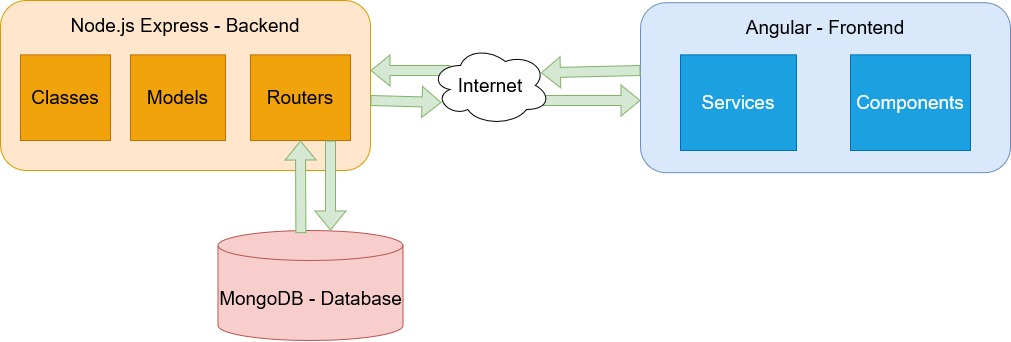
\includegraphics[scale=0.45]{images/DoubleOut_Network.drawio.png}
\caption{Az alkalmazáson belüli kommunikáció}
\label{fig:network}
\end{figure}

\Section{Statisztikai opciók és számításuk bemutatása}
Mint minden sportban, a dartsban is a mérkőzésekből különböző statisztikai adatok nyerhetők ki, az átlagoktól kezdve, a 180-as dobások számán át, a kiszálló dobások hatékonyságáig. Az alkalmazás fő funkciója, hogy egy adatbázisból, - amely meccsenként tartalmazza az adott meccshez tartozó dobásokat- , kiszámítja a statisztikákat. A statisztikák nem csupán mérkőzésenként kerülnek kiszámításra és megjelenítésre, hanem elérhetőek játékosonként is, ahol egy adott játékosnak az adatbázisban lévő összes mérkőzése kerül számításba.

Az alábbi pontokban azok a statisztikai elemek szerepelnek, amelyek kiszámításra kerülnek a meccsek vagy a játékosok esetében.

\begin{itemize}
\item Nyert legek száma:

Magának az eredményeknek a megjelenítése. Olyan mérkőzések esetében, amelyeket szettekre játszanak, külön megjelenítésre kerülnek az adott szettben megnyert legeknek a száma is. Egy leget az a játékos nyeri akinek a pontszámát a legkevesebb nyílból sikerül 0-ra redukálnia.
\item Átlagok (Average):

Egy játékos körönként dobott nyilainak az értéke, osztva a körök a számával.
\item Kiszálló dobások hatékonysága (Checkout%):

A kiszálláshoz szükséges sikeresen eldobott nyilak, és a kiszállóra összesen eldobott nyilak arányát mutatja.
\item 180-as dobások száma (180's):

Azon dobások száma játékosonként, amely elérte az egy körben dobható maximális pontszámot, azaz a 180-at.
\item 140 feletti dobások száma (140+):

Azon dobások száma játékosonként, amelynek az értéke 140 vagy annál több, de kevesebb, mint 180.
\item 100 feletti dobások száma (100+):

Azon dobások száma játékosonként, amelynek az értéke 100 vagy annál több, de kevesebb, mint 180.
\item Legmagasabb kiszálló (Highest Checkout):

Egy játékos legmagasabb pontszámú, és kiszállást is érő dobása egy meccsen.
\item Első 9 nyíl átlaga (First 9 averages):

Egy játékos első 3 körének, azaz az eldobott első 9 nyilának az átlaga.
\item Első, második és harmadik nyíl átlag értéke (First-, Second-, Third Dart Average):

Egy játékos által körönként eldobott első, második és harmadik nyilak értékeinek az átlaga.
\item Sikeres egy, kettő, és három nyilas kiszállók száma (1-, 2-, 3 Darts Checkouts):

Számontartja, hogy a játékos sikeres kiszálló dobásaihoz egy, kettő, vagy esetleg három nyíl volt szükséges.
\item Eltalált tripla 20-ak száma (Triple 20s):

Egy játékos összes olyan dobásának a száma, amellyel a játékos a tripla 20-as szektort találta el, azaz az egy nyílból dobható maximális értéket.

\item Körönként dobott 180-ak aránya (180/Leg):

Egy játékos 180-as dobásainak a száma osztva minden általa elvégzett körrel.

\end{itemize}

\Section{Az oldalak tervezése}
Az alkalmazás több oldalból áll, de természetesen az oldalak között egyszerű az átjárhatóság. Ez a fejlécnek is köszönhető ahol, a menüpontokban az összes oldal megtalálható és a fejléc természetesen minden oldalon elérhető.

Az oldal emblémájára kattintva érhetjük el a kezdő oldalt, mellette pedig menüpontokban szerepelnek a felhasználói adatlap, a játékosok, és a versenyek oldalaira irányító gombok. A versenyek a játékosok és a mérkőzések külön adatlapokat kaptak, amelyek szintén külön oldalon érhetőek el.

\subsection{Kezdő oldal}
A kezdő oldallal (\ref{fig:home} ábra) egyből az alkalmazás megnyitásakor találkozunk, itt jelennek meg a még folyamatban lévő versenyek külön blokkokban. A blokkban látható a verseny neve, ez alatt kiírásra kerül még, hogy jelenleg milyen fázisban jár, és a mellette található „Continue” gombbal az adatlapjára ugrunk, ahonnan folytatni tudjuk a versenyt a hátralévő mérkőzések lejátszásával.

Amennyiben a felhasználó nem indított még versenyt vagy csak éppen nincsen lezáratlan versenye, akkor ezek a blokkok nem jelennek meg. Azonban a kezdő oldalon megtalálható „+ New Tournament” gomb megnyomásával tudunk változtatni ezen az állapoton egy új torna létrehozásával. Itt minden szükséges adat kitöltésével létrehozható a torna, amely lezárásáig a korábban leírt módon már meg fog jelenni a kezdő oldalon is.

\begin{figure}[h]
\centering
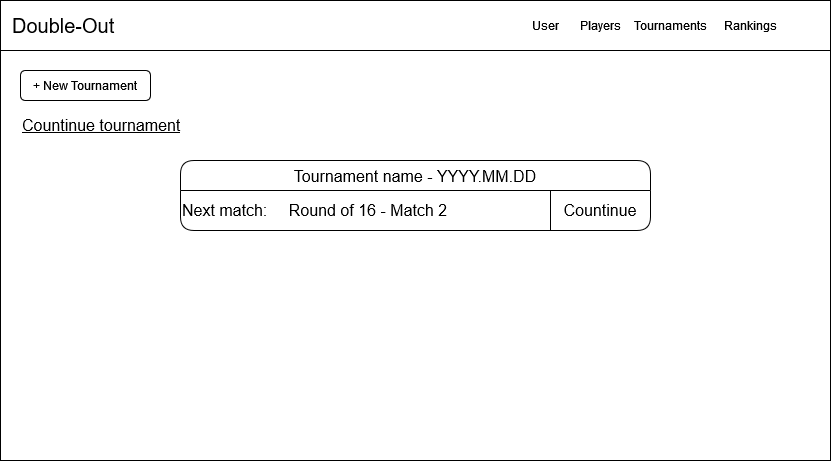
\includegraphics[scale=0.5]{images/HomePage.png}
\caption{A kezdő oldal vázlata}
\label{fig:home}
\end{figure}

\subsection{Versenyek oldala}
A versenyek oldalán (\ref{fig:tournaments} ábra) tekinthetjük meg a még zajló és a már lezárult versenyeket is. A különböző versenyek külön blokkokban jelennek meg, ezek a blokkok pedig a versenyek egyes alapvető adatait tartalmazzák, mint például a nevüket és a verseny aktuális állapotát. Az itt megtalálható „Continue” gombra kattintva az oldal tovább irányít minket a kiválasztott verseny adatlapjára.

A kezdőoldalhoz hasonlóan itt is megtalálható egy gomb az új versenyek létrehozásához, amely a verseny létrehozás oldalára irányít át. 

\begin{figure}[h]
\centering
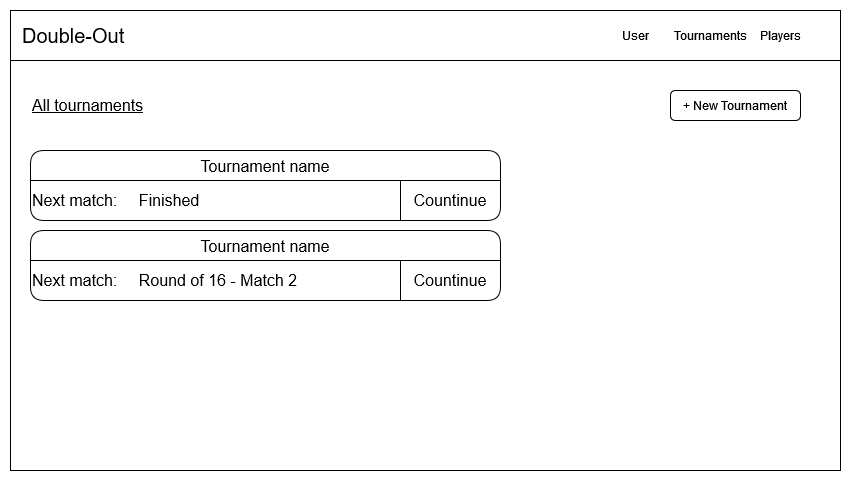
\includegraphics[scale=0.5]{images/Tournaments.png}
\caption{A versenyek oldalának vázlata}
\label{fig:tournaments}
\end{figure}

\subsection{Verseny oldal}
A verseny oldalon (\ref{fig:tournament} ábra) a kiválasztott verseny adatlapját tekinthetjük meg. Az adatlap tartalmazza a verseny mérkőzéseit és a verseny összesített statisztikáját. A mérkőzéseken keresztül tovább tudunk lépni a kiválasztott mérkőzés oldalára.

\begin{figure}[h]
\centering
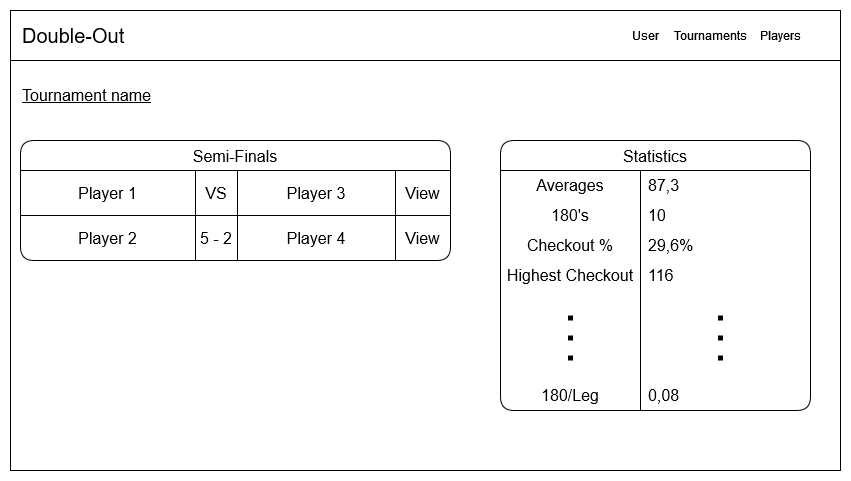
\includegraphics[scale=0.5]{images/TournamentPage.png}
\caption{A verseny oldal vázlata}
\label{fig:tournament}
\end{figure}

\subsection{Verseny létrehozása oldal}
A verseny létrehozása oldalán (\ref{fig:newTournament} ábra) van lehetőségünk egy új verseny létrehozására. Ehhez az adatok kitöltése szükséges, ami a verseny típusát határozza meg, ezt követően az „Add Players” gombbal tudunk játékosokat hozzáadni a versenyhez. Miután a minden szükséges adatot megfelelően kitöltöttünk a „Create Tournament” gombra kattintva létrehozzuk a versenyt.

\begin{figure}[h]
\centering
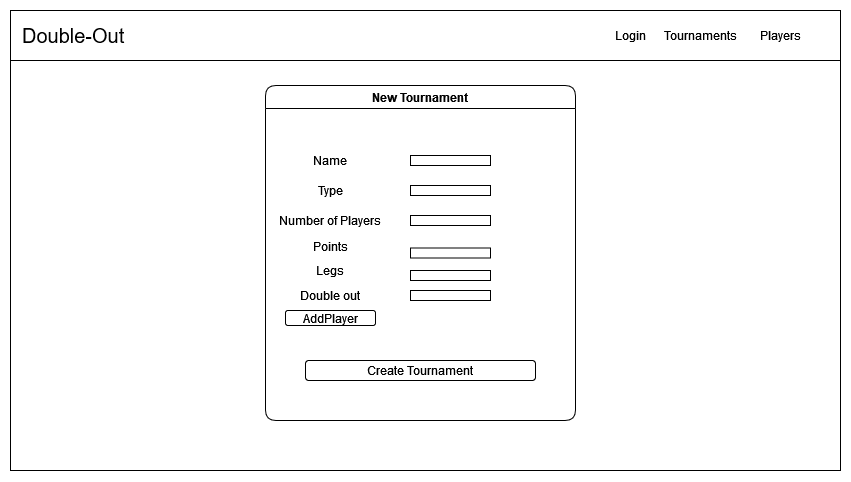
\includegraphics[scale=0.5]{images/NewTournament.png}
\caption{A verseny létrehozása oldal vázlata}
\label{fig:newTournament}
\end{figure}

\subsection{Játékosok oldala}
A játékosok oldalán (\ref{fig:players} ábra) az alkalmazásban létrehozott versenyeken résztvevő játékosok találhatók meg, illetve a neveik alapján lehetőség van keresni is közöttük. Egy adott játékost kiválasztva a játékos adatlapját tudjuk elérni egy új oldalon.

\begin{figure}[h]
\centering
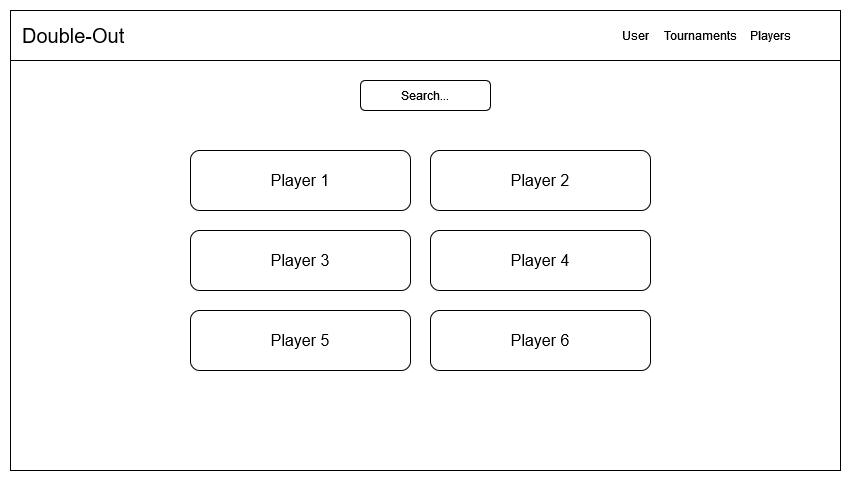
\includegraphics[scale=0.5]{images/PlayersPage.png}
\caption{A játékosok oldalának vázlata}
\label{fig:players}
\end{figure}

\subsection{Játékos oldal}
Minden játékos saját adatlappal (\ref{fig:player} ábra) rendelkezik, ahol az adott játékos statisztikáit tudjuk megtekinteni a már korábban is leírt szempontok szerint.
Emellett megtekinthetőek a játékos által lejátszott mérkőzések eredményei is.

\begin{figure}[h]
\centering
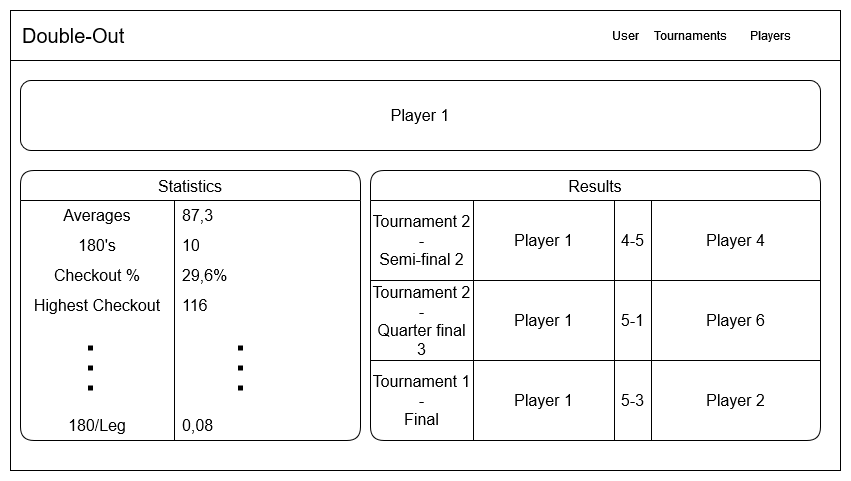
\includegraphics[scale=0.5]{images/PlayerPage.png}
\caption{A játékos oldal vázlata}
\label{fig:player}
\end{figure}

\subsection{Mérkőzés oldal}
A mérkőzés oldal (\ref{fig:match} ábra) tartalmazza a játékhoz szükséges pont kalkulátort amelybe a dobott pontokat tudjuk beírni az eltalált szektor és a szektoron belül eltalált terület megadásával, ami alapján kiszámításra kerül a dobás értéke, ami a játék szabályai alapján kivonódik a játékos pontjaiból és ez a folyamat addig ismétlődik, amíg valamelyik játékos meg nem nyeri a mérkőzést. A játékosok nevei mellett látható a mérkőzés eddigi eredménye, valamint az aktuális legen belüli pontszámaik.

Ezekből a megadott adatokból kerülnek kiszámításra a statisztikák, amelyeket szintén ezen az oldalon tekinthetünk meg, középen a statisztikai szempontokkal, a két szélén pedig a két játékos statisztikáival.

\begin{figure}[h]
\centering
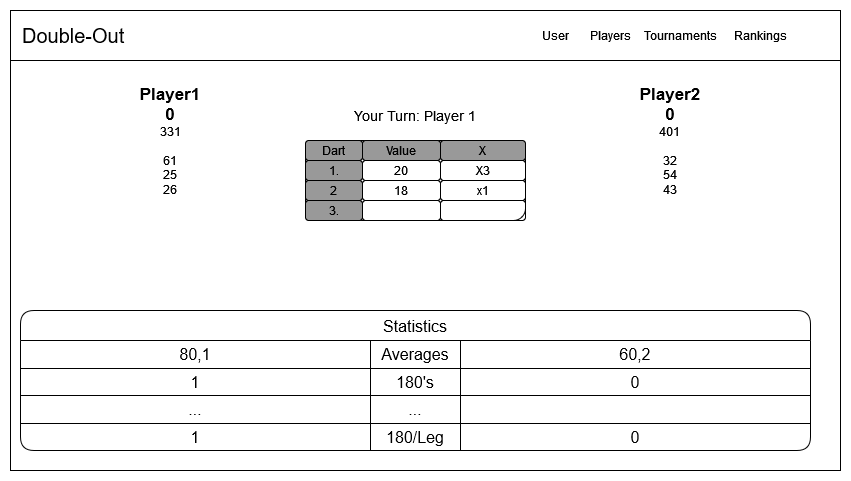
\includegraphics[scale=0.5]{images/MatchPage.png}
\caption{A mérkőzés oldal vázlata}
\label{fig:match}
\end{figure}

\subsection{Bejelentkezési oldal}
A bejelentkezési (\ref{fig:login} ábra) oldalon a korábban már regisztrált felhasználók tudnak bejelentkezni az e-mail címük és a jelszavuk megadásával.

\begin{figure}[h]
\centering
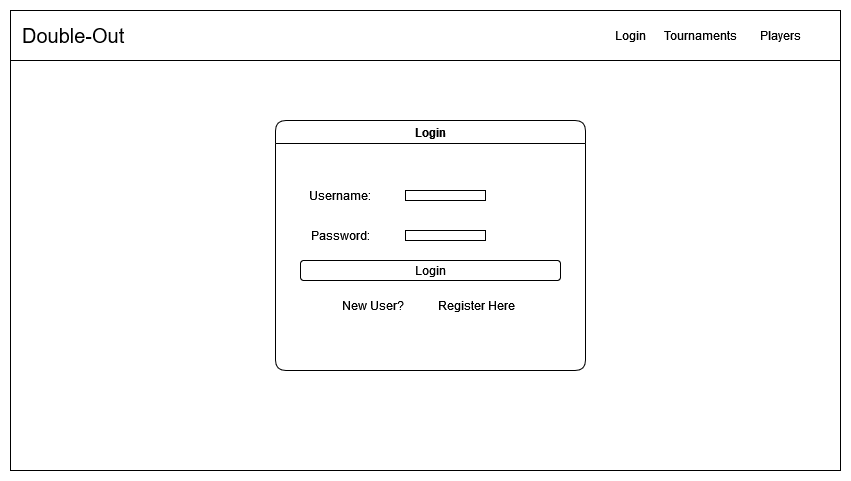
\includegraphics[scale=0.5]{images/Login.png}
\caption{A bejelentkezési oldal vázlata}
\label{fig:login}
\end{figure}

\subsection{Regisztrációs oldal}
A regisztrációs (\ref{fig:register} ábra) oldalon azon felhasználók regisztrálhatnak, akik korábban még nem tették meg. Itt egy felhasználónév, e-mail cím, és egy jelszó megadása szükséges a sikeres regisztrációhoz.

\begin{figure}[h]
\centering
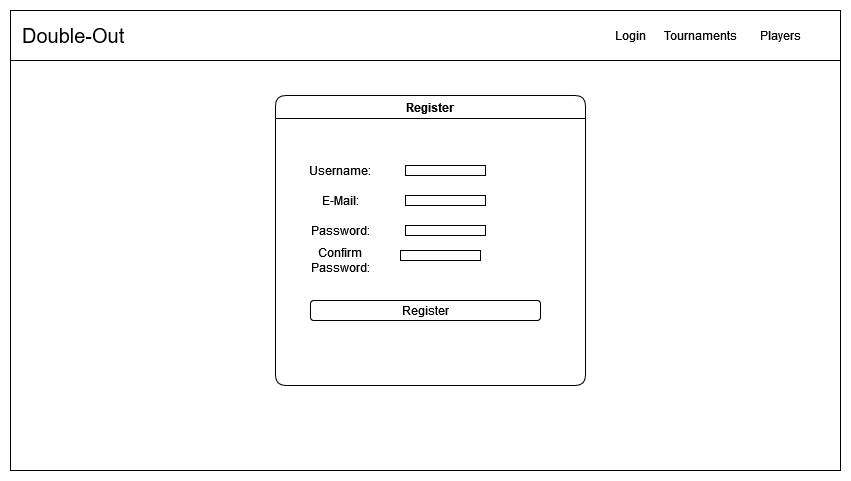
\includegraphics[scale=0.5]{images/Register.png}
\caption{A regisztrációs vázlata}
\label{fig:register}
\end{figure}

\Section{Adatmodellek bemutatása}
A program megírása során külön adatmodelleket hoztam létre a játékosok, a versenyek, a mérkőzések, a statisztikák illetve a felhasználók számára. Az alkalmazás ezen adatmodellek alapján képes az adatok feldolgozására és azok küldésére az adatbázis számára, illetve fogadására is az adatbázis irányából. A \ref{fig:graph} -es ábrán látható gráf vázolja az alkalmazás felépítését az adatmodellek szempontjából. Egy felhasználó képes létrehozni egy versenyt, amely hivatkozza a játékosokat, illetve a mérkőzéseket, az utóbbiból a statisztikák származnak, mivel azok a mérkőzés adatai alapján kerülnek kiszámításra.

\begin{figure}[h]
\centering
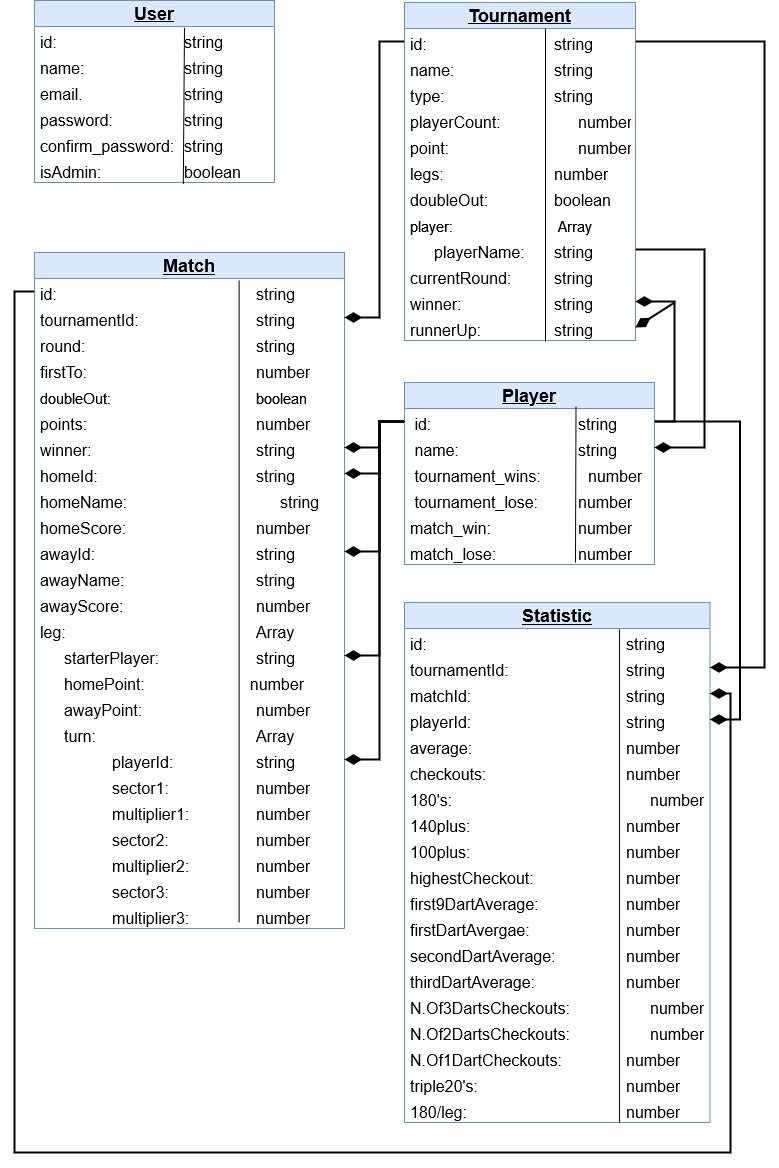
\includegraphics[scale=0.45]{images/DoubleOut_Graph.png}
\caption{Az adatbázis felépítésének vázlata}
\label{fig:graph}
\end{figure}

\subsection{User modell}
A \textit{User} modell a felhasználók adatainak a tárolására hivatott. A felépítése egyszerű, tartalmaz \textit{egy egyedi azonosítót, nevet, email címet, jelszót,} illetve egy \textit{"isAdmin"} és egy \textit{token} adattagot. Az azonosítót az adatbázis generálja a létrehozáskor, a további adatokat pedig a regisztrációkor adjuk meg. A sikeres regisztráció után ezek az adatok mentésre kerülnek az adatbázisban és a későbbiekben már lehetősége lesz a felhasználónak bejelentkezni az oldalra ezen adatok megadásával.

\begin{cpp}
export const UserSchema = new Schema<User>(
{
    name: {type: String, required: true},
    email: {type: String, required: true, unique: true},
    password: {type: String, required: true},
    isAdmin: {type: Boolean, required: true},
}, {
    timestamps: true,
    toJSON: {
        virtuals: true
    },
    toObject: {
        virtuals: true
    }
});
\end{cpp}

\subsection{Tournament modell}
A \textit{Tournament} modell képzi az alkalmazáson belüli adatmodellek alapját, mivel a verseny létrehozásától függ a játékosok és mérkőzések létrehozása is. Az adatmodell tartalmazza a \textit{verseny azonosítóját, a nevét, a típusát a játékosok számát, a mérkőzések kezdőpontszámát, a győzelemhez szükséges legek számát, a kiszálló típusát, valamint a verseny győztesének és második helyezettjének azonosítóját}. A résztvevő játékosok neveit a \textit{players} interfész segítségével tudjuk megadni.

\begin{cpp}
export const TournamentSchema = new Schema<Tournament>(
  {
    name: {type: String, required: true},
    type: {type: String, required: true},
    playersCount: {type: Number, required: true},
    points: {type: Number, required: true},
    legs: {type: Number, required: true},
    doubleOut: {type: Boolean, required: true},
    players: [
      {
        playerName: {type: String, required: true },
      },
    ],
    currentRound: {type: String, required: true },
    winner: {type: String, required: false },
    runnerUp: {type: String, required: false },
  },
  {
    toJSON: {
      virtuals: true,
    },
    toObject: {
      virtuals: true,
    },
    timestamps: true,
  }
);
\end{cpp}

\subsection{Player modell}
A versenyeken résztvevő játékosok adatait a \textit{Player}  modell segítségével tároljuk. Ez az adatmodell is viszonylag egyszerű felépítésű, az adott \textit{játékos azonosítóját, a nevét illetve a verseny és mérkőzés mérlegét tárolja, vagyis a játékos győztes, illetve vesztes mérkőzéseinek és versenyeinek a számát}.

\begin{cpp}
export const PlayerSchema = new Schema<Player>(
    {
        name: {type: String, required: true},
        tournament_win: {type: Number, required: true},
        tournament_lose: {type: Number, required: true},
        match_win: {type: Number, required: true},
        match_lose: {type: Number, required: true},
    },{
        toJSON: {
            virtuals:true
        },
        toObject: {
            virtuals: true
        },
        timestamps: true
    }
);
\end{cpp}

\subsection{Match modell}
A \textit{Match} modell segítségével tudjuk tárolni a lejátszott mérkőzések adatait, a \textit{mérkőzés azonosítójától} kezdve, az utolsó eldobott \textit{nyíl értékéig}. Az adatmodell elsősorban tartalmazza a \textit{mérkőzés azonosítóját és annak a versenynek az azonosítóját, amelynek a keretei között lejátszásra kerül a mérkőzés}. Emellett nyilvántartjuk még, hogy a mérkőzés a verseny melyik \textit{fordulójában} került lejátszásra, \textit{a kiszálló típusát} (duplával kell-e kiszállni vagy sem) és az egymás ellen játszó két \textit{játékos adatait}, vagyis az \textit{azonosítójukat, a nevüket, és az eredményüket}. Magát a mérkőzés menetét az adatmodellen belül a \textit{Leg} interfészben tároljuk, amely a nevéből adódóan a lejátszott \textit{legek adatait} tartalmazza, mint például, hogy \textit{hányadik legben járunk, ki a kezdő játékos és ki nyerte a leget}. Ezen belül található meg \textit{Turn} interfész amely a \textit{körönkénti dobásokat} tárolja, vagyis, hogy \textit{ki dobta azt a kört, illetve, hogy mennyi volt az első, a második és a harmadik nyíl értéke}. Ezeken keresztül folyik le egy mérkőzés a megadott szabályok alapján és értelemszerűen az olyan adattagok, mint a mérkőzés győztese, a leg győztese és a két játékos eredménye ezekből származik.

\begin{cpp}
export const NewMatchSchema = new Schema<Match>(
  {
    tournamentId: {type: String, required: true},
    round: {type: String, required: true},
    firstTo: {type: Number, required: true},
    doubleOut: {type: Boolean, required: true},
    points: {type: Number, required: true},
    winner: {type: String, required: false},
    homeId: {type: String, required: true},
    homeName: {type: String, required: true},
    homeScore: {type: Number, required: true},
    awayId: {type: String, required: true},
    awayName: {type: String, required: true},
    awayScore: {type: Number, required: true},
    legs: [
      {
        starterPlayer: {type: String, required: true},
        homePoint: {type: Number, required: true},
        awayPoint: {type: Number, required: true},
        winner: {type: String, required: true},
        turns: [
          {
            playerId: {type: String, required: false},
            throw1Sector: {type: Number, required: false},
            throw1Multiplier: {type: Number, required: false},
            throw2Sector: {type: Number, required: false},
            throw2Multiplier: {type: Number, required: false},
            throw3Sector: {type: Number, required: false},
            throw3Multiplier: {type: Number, required: false},
          },
        ],
      },
    ],
  },
  {
    toJSON: {
      virtuals: true,
    },
    toObject: {
      virtuals: true,
    },
    timestamps: true,
  }
);
\end{cpp}

\subsection{Stat modell}
A \textit{Stat} modell a korábban már említett szempontok szerint tárolja a játékosok statisztikáit mérkőzésenként, vagyis egy mérkőzéshez két statisztika tartozik, ami a két játékosé, egy játékoshoz pedig annyi statisztikai tartozik amennyi mérkőzésen részt vett. Amennyiben egy játékos statisztikáit szeretnénk kimutatni, akkor minden olyan eltárolt statisztikát kell összesítenünk, amelyben az ő azonosítója szerepel, és a versenyek statisztikáinak a kimutatásához ugyanígy összesítenünk kell az adatokat, csak itt a verseny azonosítója alapján.

\begin{cpp}
export const StatSchema = new Schema<Stat>(
  {
    tournamentId: {type: String, required: true},
    matchId: {type: String, required: true},
    playerId: {type: String, required: true},
    average: {type: Number, required: true},
    checkouts: {type: Number, required: true},
    numberOf180s: {type: Number, required: true},
    numberOf140plus: {type: Number, required: true},
    numberOf100plus: {type: Number, required: true},
    highestCheckout: {type: Number, required: true},
    first9DartsAverage: {type: Number, required: true},
    firstDartAvergrage: {type: Number, required: true},
    secondDartAverage: {type: Number, required: true},
    thirdDartAverage: {type: Number, required: true},
    numberOf3DartCheckouts: {type: Number, required: true},
    numberOf2DartCheckouts: {type: Number, required: true},
    numberOf1DartCheckouts: {type: Number, required: true},
    triple20s: {type: Number, required: true},
    percentageOf180PerLeg: {type: Number, required: true},
  },
  {
    toJSON: {
      virtuals: true,
    },
    toObject: {
      virtuals: true,
    },
    timestamps: true,
  }
);
\end{cpp}

\Section{Az alkalmazás végpontjai}
Az alkalmazáson belül különböző végpontok segítségével jön létre a kommunikáció. A végpontok segítségével különböző kéréseket tudunk küldeni, az alábbiakban pedig ezeket szeretném bemutatni.
\subsection{User végpontok}
A felhasználók (\ref{fig:userEndpoint} ábra) esetében az alkalmazás két Post kérést használ, amelyek segítségével a jelenlegi felhasználókkal bejelentkezhetünk, valamint új felhasználókat hozhatunk létre regisztráció által.

\begin{figure}[h]
\centering
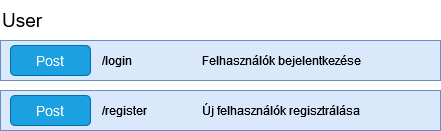
\includegraphics[scale=0.7]{images/User_Vegpontok.drawio.png}
\caption{A felhasználók által használt végpontok}
\label{fig:userEndpoint}
\end{figure}

\subsection{Player végpontok}
A játékosok (\ref{fig:playerEndpoint} ábra) három Get kérést alkalmaznak. Az első Get kérés által lekérdezünk minden olyan Objektumot az adatbázisból, ami Player típusú. A második Get kéréssel ezen objektumok között keressük meg azt az egyet, ami a megadott azonosítóval rendelkezik. Végezetül a harmadik Get kéréssel megkeresünk minden olyan Player objektumot az adatbázisban, amelynek a neve tartalmazza a keresési feltételnek megadottakat.

\begin{figure}[h]
\centering
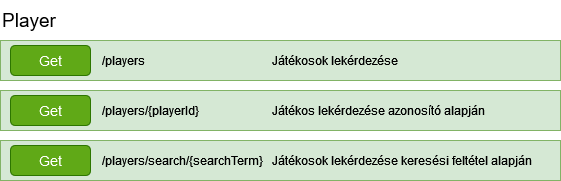
\includegraphics[scale=0.7]{images/Player_Vegpontok.drawio.png}
\caption{A játékosok által használt végpontok}
\label{fig:playerEndpoint}
\end{figure}

\subsection{Tournament végpontok}
A versenyek (\ref{fig:tournamentEndpoint} ábra) a játékosokhoz hasonlóan szintén alkalmaznak 2 Get kérést a lekérdezésekre. Az egyik Get kérés az összes verseny lekérdezésére hivatott, míg a másik megkeresi megadott azonosítóval rendelkező Player objektumot. Emellett itt megtalálható még egy Post kérés, ami által új versenyt, vagyis új Tournament objektumot rögzíthetünk az adatbázisban.

\begin{figure}[h]
\centering
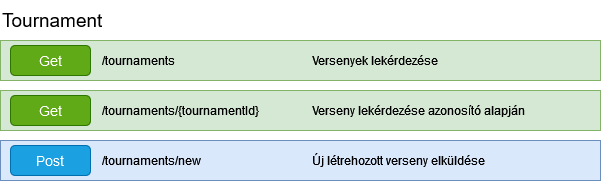
\includegraphics[scale=0.7]{images/Tournament_Vegpontok.drawio.png}
\caption{A versenyek által használt végpontok}
\label{fig:tournamentEndpoint}
\end{figure}

\subsection{Match végpontok}
A mérkőzések (\ref{fig:matchEndpoint} ábra) esetében két Get kéréssel tudjuk lekérdezni az összes mérkőzést, valamint a keresett mérkőzést az azonosítója alapján. A harmadik Get kéréssel a még be nem fejezett mérkőzéseket tudjuk folytatni. Ezek mellett a két Put kérés a mérkőzések elindításáért felelős, valamint dobások végrehajtásáért. Ezáltal a két kérés által rögzítjük és frissítjük az adott mérkőzéshez tartozó legeket és dobásokat az adatbázisban.

\begin{figure}[h]
\centering
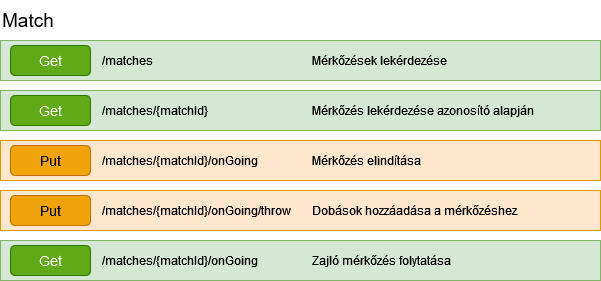
\includegraphics[scale=0.7]{images/Merkozes_Vegpontok.drawio.png}
\caption{A mérkőzések által használt végpontok}
\label{fig:matchEndpoint}
\end{figure}